% **************************************************************************** %
%                                                                              %
%                                                         :::      ::::::::    %
%    sec_resultados.tex                                 :+:      :+:    :+:    %
%                                                     +:+ +:+         +:+      %
%    By: acampo-p <acampo-p@student.42urduliz.com>  +#+  +:+       +#+         %
%                                                 +#+#+#+#+#+   +#+            %
%    Created: 2022/12/07 17:42:28 by acampo-p          #+#    #+#              %
%    Updated: 2023/02/16 03:42:11 by acampo-p         ###   ########.fr        %
%                                                                              %
% **************************************************************************** %

\section{RESULTADOS}

Una vez el modelo de la simulación ha sido finalizado,
los siguientes escenarios expuestos en la Tabla~\ref{tab:4_tbl_scenes}
han sido simulados mediante el cambio de sus respectivas variables de entrada
expuestas en las Tablas~\ref{tab:3_tbl_sim_det} y \ref{tab:3_tbl_rsrc}.
Cada escenario ha sido ejecutado 100 veces.

\begin{table}[h]
	\centering
	\caption{Listado de los escenarios simulados.}
	\documentclass[varwidth=\maxdimen]{standalone}
\usepackage[utf8]{inputenc}
\usepackage[spanish]{babel}
\usepackage{booktabs}
\usepackage{tabularx}

\begin{document}

\begin{tabularx}{\textwidth}{ l l X }
	\toprule
	ID & Variable alterada	& Descripción \\
	\midrule
	E0	& Ninguna	& Escenario original\\
	\addlinespace
	T2	& Turnos	& 1 técnico añadido trabajando a relevos. 16 horas de técnico disponible diariamente de lunes a viernes. \\
	T3	&			& 2 técnicos añadidos trabajando a relevos. 24 horas diarias de técnico disponible de lunes a viernes. \\
	T4	&			& 3 técnicos añadidos trabajando a relevos. Técnico disponible 24 horas 365 días al año. \\
	\addlinespace
	W2	& Técnicos	& 1 técnico añadido que trabaja simultáneamente al existente. La función de este técnico es dar soporte al primero \\
	\addlinespace
	M1	& Máquinas \textit{Endurance} & 1 sola máquina \textit{Endurance} instalada en el laboratorio. \\
	M2	&  			& 2 máquinas \textit{Endurance} instaladas en el laboratorio. \\
	M3	& 			& 3 máquinas \textit{Endurance} instaladas en el laboratorio. \\
	M5	& 			& 5 máquinas \textit{Endurance} instaladas en el laboratorio. \\
	M10	& 			& 10 máquinas \textit{Endurance} instaladas en el laboratorio. \\
	\bottomrule
\end{tabularx}
\end{document}

	\label{tab:4_tbl_scenes}
\end{table}

A continuación,
se ha procedido a analizar las tablas de datos obtenidos por las simulaciones.

En la Figura~\ref{fig:4_hist_tests_done} se han graficado
las distribuciones del número de ensayos realizados, en un año simulado,
para los escenarios \textit{E0}, \textit{T2}, \textit{T3} y \textit{T4}.
Se ha trazado la frecuencia
con la que ocurría un determinado número de ensayos en el histograma.
En el eje $X$ se representa la cantidad de ensayos realizados,
mientras que el eje $Y$ mide la cantidad de veces que se repite
un número de ensayos en el conjunto de ejecuciones obtenido.
La Figura~\ref{fig:4_hist_tests_done}A corresponde
a los ensayos \textit{Endurance},
y la Figura~\ref{fig:4_hist_tests_done}B 
a los ensayos \textit{Rolling Resistance}.

En la Figura~\ref{fig:4_hist_tests_done}A puede observarse la distinción
que ocurre entre las distintas configuraciones.
Cada uno de los escenarios tiene un amplio rango de ensayos,
mostrando el comportamiento estocástico de este tipo de ensayos.
Exceptuando el escenario \textit{T4},
la cantidad de ensayos, parece variar dentro de un rango común de 100 ensayos.
Esta tendencia cambia al disponer los 365 días del año 
de un operario que monte la máquina.
Al eliminarse la posibilidad
de que el ensayo finalice fuera del horario laboral,
la desviación estándar de ensayos realizados se reduce al mismo tiempo
que la media de ensayos se aproxima a la capacidad ideal
expuesta en la Tabla~\ref{tab:4_tbl_max_cap}.

\begin{table}[H]
	\centering
	\caption{Capacidad máxima de ensayos por máquina.}
	\documentclass[varwidth=\maxdimen]{standalone}
\usepackage[utf8]{inputenc}
\usepackage[spanish]{babel}
\usepackage{booktabs}

\begin{document}

\begin{tabular}{ l c }
	\toprule
	Ensayo & Capacidad máxima (unds.) \\
	\midrule
	\textit{Endurance}	& 934 \\
	\textit{Rolling Resistance}		& 2502 \\
	\bottomrule
\end{tabular}

\end{document}

	\label{tab:4_tbl_max_cap}
\end{table}

\begin{figure}
	\begin{center}
		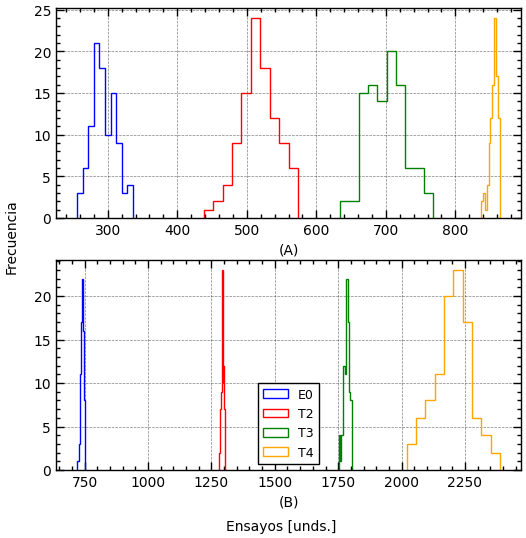
\includegraphics{fig/4_hist_tests_done}
	\end{center}
	\caption{Distribución de ensayos realizados para los escenarios descritos en la leyenda.
	(A) Ensayos \textit{Endurance}. (B) Ensayos \textit{Rolling Resistance}.}
	\label{fig:4_hist_tests_done}
\end{figure}

En la Figura~\ref{fig:4_hist_tests_done}B,
los escenarios \textit{E0}, \textit{T2} y \textit{T3},
muestran un comportamiento similar al observado en
el escenario \textit{T4} de la Figura~\ref{fig:4_hist_tests_done}A.
Esto se debe, a que en el horario de trabajo disponible,
solamente puede llegar a lanzar un determinado numero de ensayos,
debido a los descansos entre turnos.
Esta cantidad se mantiene uniforme a lo largo de las ejecuciones
gracias a que la duración de este ensayo es inferior
a la duración del horario laboral disponible.
Mientras el horario del que se disponga de un técnico sea limitado,
la tendencia de ensayos corresponderá a la ecuación~\eqref{eq:testdone}.
En el escenario \textit{T3},
la acumulación de eventos aleatorios se vuelve notable
en la desviación de ensayos observada respecto a
los escenarios \textit{E0} y \textit{T2}.
Esto se ve reflejado en la mayor dispersión de $T3$.
Finalmente, en el escenario \textit{T4}, la desviación estándar
aumenta considerablemente, ya que no hay un descanso
que regule la aleatoriedad de los ensayos.

\begin{equation}
	Test Realizados = 365 \cdot 8 \cdot 
	\underbrace{
		\left(\frac{N_{turnos}}{\mu_{test}} + 1\right)
	}_{\text{Entero truncado}}
	\label{eq:testdone}
\end{equation}

Una representación más significativa ocurre
cuando se normaliza la cantidad de ensayos respecto
a la capacidad máxima de trabajo.
La normalización se ha realizado de la siguiente manera:

\begin{enumerate}
	\item Dividir el conjunto de ensayos realizados
		obtenido como variable de salida en cada escenario
		entre la capacidad máxima de ensayos
		representada en la Tabla~\ref{tab:4_tbl_max_cap}.
		De esta manera se obtiene la fracción de
		tiempo en funcionamiento de la máquina, es decir,
		la saturación de la máquina, representada en el eje $X$.
	\item Dividir la frecuencia con la que ocurre
		un determinado rango de ensayos en una simulación
		entre el tamaño del conjunto.
		Por ejemplo, si la población del conjunto es de 100 ejecuciones,
		y se han contado un total de 10 ensayos en el grupo
		entre 250 y 300 ensayos,
		se realiza la siguiente operación $10 / 100 = 0,1$.
		De esta manera se logra la frecuencia relativa
		representada en el eje $Y$.
\end{enumerate}

Siguiendo estos pasos, se obtienen las distribuciones
de tiempo de saturación de máquina
representadas en la Figura~\ref{fig:4_hist_time_sat}.
Esta conversión logra asentar la base necesaria para
comparar el grado de utilización de máquinas de manera directa.

\begin{figure}
	\begin{center}
		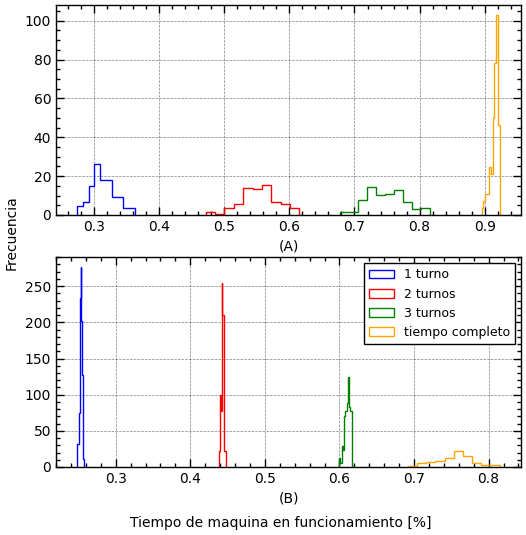
\includegraphics{fig/4_hist_time_sat}
	\end{center}
	\caption{Distribución del nivel de saturación en tiempo de lo escenarios descritos en la leyenda.
	(A) Ensayos \textit{Endurance}. (B) Ensayos \textit{Rolling Resistance}.}
	\label{fig:4_hist_time_sat}
\end{figure}

\begin{table}
	\centering
	\caption{Media y desviación estándar de ensayos realizados por cada escenario y tipo de ensayo.}
	\documentclass[varwidth=\maxdimen]{standalone}
\usepackage[utf8]{inputenc}
\usepackage[spanish]{babel}
\usepackage{booktabs}
\usepackage{multirow}

\begin{document}

\begin{tabular}{ l c c c c }
	\toprule
	Escenario &
	\multicolumn{2}{c}{Ensayos \textit{Endurance} (unds.)} &
	\multicolumn{2}{c}{Ensayos \textit{Rolling Resistance} (unds.)} \\
		& $\mu$		& $\sigma$	& $\mu$		& $\sigma$ \\
	\midrule
	E0	& 293.35    & 17.27		& 739.35	& 5.51 \\
	T2	& 516.83	& 26.38		& 1293.40	& 5.00\\
	T3	& 701.07	& 27.25		& 1782.26	& 11.15 \\
	T4	& 855.06	& 5.70		& 2202.28	& 73.18 \\
	\bottomrule
\end{tabular}

\end{document}

	\label{tab:4_tbl_test_done}
\end{table}

Si se grafica la fracción de tiempo de utilización de máquina,
respecto a la fracción del tiempo trabajado,
con los escenarios expuestos hasta ahora,
se obtiene la Figura~\ref{fig:4_sctr_time_sat}.
La dispersión de los datos se ajusta perfectamente a una regresión lineal
a partir de la fracción de tiempo trabajado de 0.25 en adelante.
Para ambas máquinas, la relación entre ensayos realizados
y tiempo trabajado es directamente proporcional.
La obtención de esta relación,
junto con las capacidades máximas de las maquinas
expuestas en la Tabla~\ref{tab:4_tbl_max_cap} permite 
anticipar si la capacidad del LCP será suficiente
para saciar la demanda de ensayos.

\begin{figure}[H]
	\begin{center}
		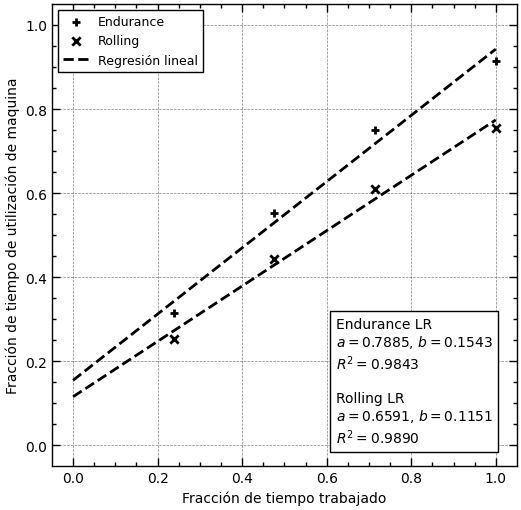
\includegraphics{fig/4_sctr_time_sat}
	\end{center}
	\caption{Tendencia proporcional del aumento del número de ensayos al añadir turnos de trabajo.}
	\label{fig:4_sctr_time_sat}
\end{figure}

Teniendo en cuenta los datos obtenidos a través de la regresión lineal,
la ecuación~\eqref{eq:qced} modela la cantidad de ensayos \textit{Endurance}
realizados en función a la fracción de horas trabajadas en un año.
Siendo la fracción de horas trabajadas descrita
como la ecuación~\eqref{eq:f_hours}.
A su vez, la ecuación~\eqref{eq:rr} aplica la misma función
a los ensayos \textit{Rolling Resistance}.
Para un determinado objetivo de test realizados,
las ecuaciones mencionadas pueden resolverse
para obtener la cantidad de horas necesarias para llegar al objetivo.
En el caso de requerir más horas de las que una jornada laboral normal dispone,
se propone completar dichas horas sobrantes
reposicionando uno de los técnicos en un turno adicional durante un periodo.
Dicho periodo se puede calcular mediante la ecuación~\eqref{eq:period},
de esta manera se aprovechan al máximo los recursos humanos disponibles.
Para ello primeramente se calcula
el máximo de turnos anuales mediante la ecuación~\eqref{eq:gf}.

\begin{equation}
	Test Realizados = 934 \cdot 0.79 \cdot f_{t trabajo} + 0.15
	\label{eq:qced}
\end{equation}

\begin{equation}
	Test Realizados = 2502 \cdot 0.66 \cdot f_{t trabajo} + 0.12
	\label{eq:rr}
\end{equation}

\begin{equation}
	f_{t trabajo}= \frac{t_{trabajo}}{365~\frac{\text{días}}{\text{año}} \cdot
	24~\frac{\text{horas}}{\text{días}}}
	\label{eq:f_hours}
\end{equation}

\begin{equation}
	\begin{array}{c}
		G(f_{t trabajo}) = f_{t trabajo}
		\frac{365~\text{días}
		\cdot 24~\frac{\text{horas}}{\text{días}}}
		{8~\frac{\text{horas}}{\text{días}} \cdot
			5~\frac{\text{días}}{\text{semanas}} \cdot
		52~\frac{\text{semanas}}{\text{año}}} \\
		\\
		Turnos= 
		\begin{cases}
			1	& G(f_{t trabajo}) \leq 1 \\
			2	& 1 < G(f_{t trabajo}) \leq 2 \\
			3	& 2 < G(f_{t trabajo}) \leq 3 \\
			4	& G(f_{t trabajo}) > 3
		\end{cases}
	\end{array}
	\label{eq:gf}
\end{equation}

\begin{equation}
	Periodo = 12~\text{meses} \cdot (G(f_{t trabajo}) - Turnos -1)
	\label{eq:period}
\end{equation}

Con el fin de descartar otro tipo de configuraciones,
como múltiples técnicos trabajando simultáneamente,
se ha graficado la Figura~\ref{fig:4_box_techn1-2_comp}.
En el gráfico se representa la distribución de los conjuntos de
tiempo de utilización de máquina para los escenarios \textit{E0} y \textit{W2}.
La Figura~\ref{fig:4_box_techn1-2_comp}A
corresponde a los ensayos \textit{Endurance},
mientras que la Figura~\ref{fig:4_box_techn1-2_comp}B
expone los ensayos \textit{Rolling Resistance}.
La diferencia en ambos ensayos parece mínima,
pero con la intención de descartar la idea de que
2 técnicos trabajando simultáneamente incrementa el numero de ensayos realizados,
se desarrolla el siguiente test de hipótesis.

\begin{itemize}
	\item $H_1$: $\mu_1 \neq \mu_2$
	\item $H_0$: $\mu_1 = \mu_2$
\end{itemize}

\begin{figure}
	\begin{center}
		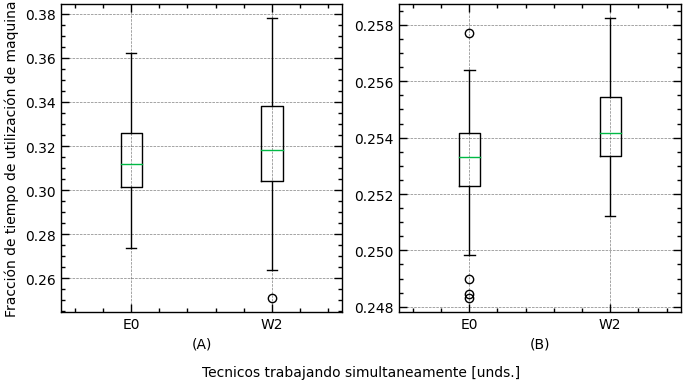
\includegraphics[width=\textwidth]{fig/4_box_techn1-2_comp}
	\end{center}
	\caption{Comparación del nivel de saturación en tiempo entre 1 técnico y 2 técnicos trabajando simultáneamente.
	(A) Ensayos \textit{Endurance}. (B) Ensayos \textit{Rolling Resistance}.}
	\label{fig:4_box_techn1-2_comp}
\end{figure}

Se ha tratado de descartar la hipótesis nula mediante la prueba de valor p,
y test t de Student.
Los resultados de la prueba,
han sido recogidos en la Tabla~\ref{tab:4_tbl_studet-t}.
Siendo el valor $p < 0,05$ en ambos tipos de ensayo
se descarta la hipótesis nula formulada anteriormente.
Esto significa que las distribuciones
tienen una diferencia estadísticamente significativa.
Aún siendo este el caso,
el escenario en el que se trabaja a 2 turnos,
es definitivamente superior,
como se puede observar en la Figura~\ref{fig:4_bar_2shift-2techn_comp}.
Al consumir ambos la misma cantidad de recursos,
esto descarta la configuración en la que 2 técnicos trabajan simultáneamente.

\begin{table}
	\centering
	\caption{Resultados del test estadístico formulado a partir de los resultados de la Figura~\ref{fig:4_box_techn1-2_comp}}
	\documentclass[varwidth=\maxdimen]{standalone}
\usepackage[utf8]{inputenc}
\usepackage[spanish]{babel}
\usepackage{booktabs}
\usepackage{multirow}

\begin{document}

\begin{tabular}{ l c c }
	\toprule
	Resultados	& Endurance	& Rolling \\
	\midrule
	valor-t		& -2.279	& -5.179 \\
	valor-p		& 0.023		& 0.000 \\
	\bottomrule
\end{tabular}

\end{document}

	\label{tab:4_tbl_studet-t}
\end{table}

\begin{figure}
	\begin{center}
		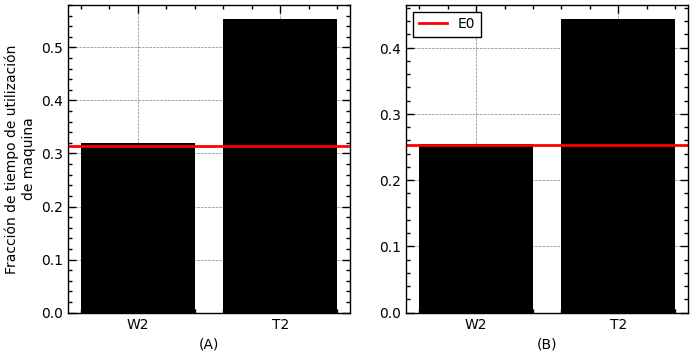
\includegraphics[width=\textwidth]{fig/4_bar_2shift-2techn_comp}
	\end{center}
	\caption{Comparación del nivel de saturación en tiempo entre los
		escenarios \textit{W2} y \textit{T2} respecto al escenario \textit{E0}.
	(A) Ensayos \textit{Endurance}. (B) Ensayos \textit{Rolling Resistance}.}
	\label{fig:4_bar_2shift-2techn_comp}
\end{figure}

Por último, se ha tratado de observar el rendimiento de ensayos
que aportaría la instalación de nuevas máquinas
para el ensayo \textit{Endurance}.
Para ello se han simulado los escenarios \textit{M1}, \textit{M2}, \textit{M3},
\textit{E0}, \textit{M5} y \textit{M10}.
A partir del conjunto de datos de cada escenario,
se ha obtenido la média de los ensayos realizados en un año para uno de ellos.
En la Figura~\ref{fig:4_sctr_indoor}, se observa como añadir máquinas
no aumenta de manera significativa la cantidad de ensayos realizados,
ya que el técnico queda saturado de trabajo con la configuración actual.

\begin{figure}[H]
	\begin{center}
	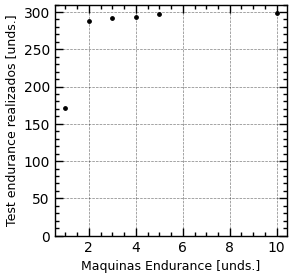
\includegraphics{fig/4_sctr_indoor}
	\end{center}
	\caption{Aumento de los ensayos realizados en función del
	número de maquinas \textit{Endurance} instaladas.}
	\label{fig:4_sctr_indoor}
\end{figure}

Este análisis concluye, que en caso de necesitar capacidad adicional,
se opte por reposicionar a uno de los técnicos
en un turno adicional durante el periodo que sea necesario.
Habiendo demostrado ser la opción óptima entre todos los escenarios simulados.
